\documentclass[10pt]{beamer}

\usepackage[spanish,activeacute]{babel}
\usepackage[utf8x]{inputenc}
\usepackage{eurosym}
\usepackage{amsmath}
\usepackage{amsfonts}
\usepackage{amssymb}
\usepackage{graphicx}
\usepackage{lmodern}
\usepackage{enumerate}



\def\X{\ve{X}}
\def\x{\ve{x}}
\newcommand{\p}[1]{p_{_{#1}}} %pdf or pmf

\definecolor{darkblue}{rgb}{0.0, 0.0, 0.55}
\setbeamercolor{title}{fg=darkblue}
\setbeamercolor{frametitle}{fg=darkblue}
\newcommand{\myitem}{\item[$\bullet$]}
\definecolor{darkgreen}{rgb}{0, 0.55, 0}
\definecolor{darkred}{rgb}{0.55, 0,0}

\usepackage{tikz}
\usetikzlibrary{fit,positioning}
\usetikzlibrary{shapes,matrix,decorations.markings,arrows}
\usetikzlibrary{graphs}
\newcommand{\ve}[1]{\boldsymbol{#1}}
\newcommand{\set}[1]{\mathcal{#1}}
    \usetikzlibrary{chains,positioning}
    \usepackage{mathtools}

\newcommand{\noteB}[1]{\textbf{\textcolor{darkblue}{#1}}}

\newcommand{\noteR}[1]{\textbf{\textcolor{darkred}{#1}}}

\newcommand{\noteG}[1]{\textbf{\textcolor{darkgreen}{#1}}}

\newcommand{\mes}[2]{m_{#1\rightarrow#2}}
\newcommand{\logmes}[2]{l_{#1\rightarrow#2}}
\newcommand{\Iset}[1]{\mathtt{#1}} %Index set

\setbeamertemplate{navigation symbols}{\usebeamerfont{footline} \insertframenumber/\inserttotalframenumber}
\logo{
\includegraphics[scale=0.04]{logouc3m.eps}}

\title{Inference in Bayesian Networks}
\author{Pablo M. Olmos, olmos@tsc.uc3m.es}
\date{Course on Bayesian Networks,  November 2016}

%\AtBeginSection{\frame{\tableofcontents[currentsection]}}
\AtBeginSection{\frame{\sectionpage}}
%\AtBeginSubsection{\frame{\subsectionpage}}
\AtBeginSubsection{\frame{\frametitle{Bayessian Networks}\tableofcontents[currentsection,currentsubsection]}}

\begin{document}

\frame{\titlepage}

\begin{frame}{Index}
\tableofcontents
\end{frame}




\section{Discrete Inference using Belief Propagation}

\begin{frame}{Discrete Inference}

\begin{itemize}
\item Let $X_j\in\set{X}$, $j=1,\ldots,5$, be discrete R.V., where $K\doteq|\set{X}|$
\item Consider the following BN:
\end{itemize}
\begin{align*}
p(\x)=p(x_1)p(x_2|x_1)p(x_4)p(x_3|x_2,x_4)p(x_5|x_4)p(x_6|x_2)
\end{align*}


\begin{figure}
\centering
\begin{tikzpicture}[scale=0.8]
\tikzstyle{factor}=[rectangle,minimum size = 3mm, thick, draw =black,fill=black]
\tikzstyle{var}=[circle,minimum size = 3mm, thick, draw =black,fill=black]
\tikzstyle{var2}=[circle, thick, draw =black]
\tikzstyle{second}=[circle, minimum size = 10mm, thick]
\tikzstyle{box}=[rectangle, draw=black!100]
\tikzstyle{connect}=[-latex, thick]
\tikzstyle{arrow}=[draw, -latex] 

\draw[step=5cm];
	\node[var2] (x_1) at (-1,0) []{$x_1$};
	\node[var2] (x_2) at (1,0) []{$x_2$};
	\node[var2] (x_3) at (3,0) []{$x_3$};
	\node[var2] (x_4) at (3,-2) []{$x_4$};
	\node[var2] (x_5) at (5,-2) []{$x_5$};
	\node[var2] (x_6) at (1,-2) []{$x_6$};
	
	\path [arrow]
		(x_1) edge []  (x_2)
		(x_2) edge []  (x_3)
		(x_2) edge []  (x_6)
		(x_4) edge []  (x_3)
		(x_4) edge []  (x_5);
				
\end{tikzpicture}
\end{figure}

\begin{itemize}
\item \textcolor{darkred}{\textbf{Inference}}: evaluate the probability distribution over some set of variables, given the
values of another set of variables.
\end{itemize}

\end{frame}

\begin{frame}{Brute-force Inference}
\begin{align*}
p(\x)=p(x_1)p(x_2|x_1)p(x_4)p(x_3|x_2,x_4)p(x_5|x_4)p(x_6|x_2)
\end{align*}
\begin{itemize}
\item Assume each variable is binary, i.e., $\set{X}=\{0,1\}$.
\item For example, how can we compute $p(x_2|x_1=0)$?
\end{itemize}

\vspace{0.5cm}
\textbf{\textcolor{darkred}{Naive approach}}:
\begin{align*}
p(x_1=0,x_2)&=\sum_{x_3,x_4,x_5,x_6} p(x_1=0,x_2,x_3,x_4,x_5,x_6) \qquad \color{darkred}{[\text{32 terms}]}\\
p(x_1=0)&=\sum_{x_2} p(x_1=0,x_2) \qquad \color{darkred}{[\text{2 terms}]} \\
p(x_2|x_1=0)&=\frac{p(x_1=0,x_2)}{p(x_1=0)} \qquad \color{darkred}{[\text{2 terms}]}
\end{align*}


\textcolor{darkblue}{The naive approach for discrete inference for $n$ R.V. each taking $K$ possible values  has complexity $\mathcal{O}\left(K^n\right)$.}

\end{frame}



\begin{frame}{A more efficient approach}
\begin{align*}
p(\x)=p(x_1)p(x_2|x_1)p(x_4)p(x_3|x_2,x_4)p(x_5|x_4)p(x_6|x_2)
\end{align*}

The \textcolor{darkgreen}{Variable Elimination} method exploits the factorization of $p(\x)$ and distributive law to efficiently compute marginals.
\begin{align*}
&p(x_1=0,x_2)=\sum_{x_3,x_4,x_5,x_6} p(x_1=0,x_2,x_3,x_4,x_5,x_6)\\
&=p(x_1=0)p(x_2|x_1=0)\left(\sum_{x_6} p(x_6|x_2)\right) \left(\sum_{x_3,x_4} p(x_4)p(x_3|x_2,x_4) \sum_{x_5} p(x_5|x_4) \right)
\\
&=p(x_1=0)p(x_2|x_1=0)\underbrace{\sum_{x_3,x_4} p(x_4)p(x_3|x_2,x_4)}_{f(x_2)} \qquad \color{darkred}{[\text{8 terms}]}
\end{align*}
\end{frame}

\begin{frame}{Re-using computations}
\begin{align*}
p(\x)=p(x_1)p(x_2|x_1)p(x_4)p(x_3|x_2,x_4)p(x_5|x_4)p(x_6|x_2)
\end{align*}
\begin{itemize}
\item Imagine we are also interested in computing $p(x_1=0,x_6)$.
\end{itemize}
\begin{align*}
&p(x_1=0,x_6)=\sum_{x_2,x_3,x_4,x_5} p(x_1=0,x_2,x_3,x_4,x_5,x_6)\\
&=p(x_1=0)\sum_{x_2}p(x_6|x_2) p(x_2|x_1=0) \underbrace{\left(\sum_{x_3,x_4} p(x_4)p(x_3|x_2,x_4)\right)}_{f(x_2) }
\end{align*}
\begin{itemize}
\item Storing Intermediate computations (such as $f(x_2)$) makes infernce very efficient if multiple queries are made over $p(\x)$.
\item \textcolor{darkblue}{Belief Propagation}! 
\end{itemize}
\end{frame}

\begin{frame}{Factor graphs}
\begin{itemize}
\item In inference,  it’s often easier to convert directed and
undirected graphs into factor graphs.
\end{itemize}
\begin{align*}
p(\x)&=p(x_1)p(x_2|x_1)p(x_4)p(x_3|x_2,x_4)p(x_5|x_4)p(x_6|x_2)\\
&=t_1(x_1)t_2(x_1,x_2)t_3(x_2,x_3,x_4)t_4(x_4)t_5(x_4,x_5)t_6(x_2,x_6)
\end{align*}


\begin{figure}
\centering
\begin{tikzpicture}[scale=0.8]
\tikzstyle{factor}=[rectangle,minimum size = 3mm, thick, draw =black,fill=black]
\tikzstyle{var}=[circle,minimum size = 3mm, thick, draw =black,fill=black]
\tikzstyle{second}=[circle, minimum size = 10mm, thick]
\tikzstyle{box}=[rectangle, draw=black!100]
\tikzstyle{connect}=[-latex, thick]
\draw[step=5cm];

	\node[factor] (t_1) at (-2,0) [label=above:{$t_1$}]{};
	\node[var] (x_1) at (-1,0) [label=above:{$x_1$}]{};
	\node[factor] (t_2) at (0,0) [label=above:{$t_2$}]{};
	\node[var] (x_2) at (1,0) [label=above:{$x_2$}]{};
	\node[factor] (t_3) at (2,0) [label=above:{$t_3$}]{};
	\node[var] (x_3) at (3,1) [label=above:{$x_3$}]{};
	\node[factor] (t_4) at (3,-2) [label=below:{$t_4$}]{};
	\node[var] (x_4) at (3,-1) [label=left:{$x_4$}]{};
	\node[factor] (t_5) at (4,-1) [label=below:{$t_5$}]{};
	\node[var] (x_5) at (5,-1) [label=right:{$x_5$}]{};
	\node[factor] (t_6) at (1,-1) [label=left:{$t_6$}]{};
	\node[var] (x_6) at (1,-2) [label=below:{$x_6$}]{};
	
	
%     \node[] () at (7,1) [label=right:{$\Iset{Ne}(X_4)=\{2,4,5\}$}]{};
%	\node[] () at (7,-1) [label=right:{$\Iset{Ne}(t_2)=\{2,4,3\}$}]{};

	\path
		(t_1) edge []  (t_3)
		(x_2) edge [] (x_6) 
		(t_3) edge [] (x_3) 
		(t_3) edge [] (x_4)
		(x_4) edge [] (t_4)
		(x_4) edge [] (x_5);
		
\end{tikzpicture}
\end{figure}



\begin{itemize}
\item \textcolor{darkblue}{Variables nodes}: we draw  circles for each variable $X_i$ in the distribution.
\item \textcolor{darkblue}{Factor nodes}: we draw filled dots for each factor $t_j$ in the distribution.
\end{itemize}

\end{frame}

\begin{frame}{Belief Propagation (I)}
\begin{itemize}
\item Local computations are regarded as \emph{messages}  between the nodes in the factor graph.
\item Iterative message-passing algorithm.
\item \noteB{$\mes{x_i}{t_j}(x_i)$} denotes the message sent from node $X_i$ to factor node $t_j$.
\item \noteB{$\mes{t_j}{x_i}(x_i)$} denotes the message sent from factor node $t_j$ to variable node $X_i$.
\item Both  messages are indeed functions of $X_i$, namely each message is a stored table of $|\set{X}|$ values.
\item At each iteration, messages are updated following simple \noteB{update rules} according to a valid \noteG{schedule}.
\end{itemize}

\end{frame}

\frame{
\frametitle{Update rules (I)}
\begin{tikzpicture}[scale=0.7]
\tikzstyle{factor}=[rectangle,minimum size = 3mm, thick, draw =black, node distance = 16mm,fill=black]
\tikzstyle{var}=[circle,minimum size = 3mm, thick, draw =black, node distance = 16mm,fill=black]
\tikzstyle{second}=[circle, minimum size = 10mm, thick, node distance = 5mm]
\tikzstyle{box}=[rectangle, draw=black!100]
\tikzstyle{connect}=[-latex, thick]
\node[second] at (-6,2) [label=center:{\textbf{Variable-to-factor message}}]{};
\node[second] at (-6,0) [label=center:{$\displaystyle\mes{x_i}{t_j}(x_i)=\prod_{\substack{k\in\Iset{Ne}(X_i) \\ k\neq j}}\mes{t_k}{x_i}(x_i)$}]{};
%\node[second] at (-6,-2) [label=center:{\color{darkred}{$|\Iset{Ne}(X_i)|\times |\set{X}|$ pointwise multiplications}}]{};

\node[factor] (t_1) at (1,2) [label=above:$t_1$]{};
\node[factor] (t_2) at (0,0) [label=above:$t_2$]{};
\node[factor] (t_3) at (1,-2) [label=above:$t_3$]{};
\node[var] (x_i) at (2.5,0) [label=above:$X_i$]{};
\node[factor] (t_j) at (5,0) [label=above: $t_j$]{};
\node[second] (m1i) at (1,1.25) [label=right: $\mes{t_1}{x_i}$]{};
\node[second] (m2i) at (1,-1.25) [label=right: $\mes{t_3}{x_i}$]{};
\node[second] (m3i) at (-0.5,0.2) [label=right: $\mes{t_2}{x_i}$]{};
\node[second] (m4i) at (2,0.2) [label=right: $\mes{x_i}{t_j}$]{};

\path
	(t_1) edge (x_i)
	(t_2) edge (x_i)
	(t_3) edge (x_i)
	(x_i) edge (t_j);
%
%\node[second] at (-6,-4) [label=center:{\textcontinuedbf{Factor-to-variable message}}]{};
%\node[second] at (-6,-6) [label=center:{$\displaystyle\mes{t_j}{x_i}(x_i)=\sum_{\x_{j}\sim x_i}~ t_j(\x_{j})\prod_{\substack{m\in \Iset{Ne}(t_j) \\ m\neq i}}\mes{x_m}{t_j}(x_m)$}]{};
%%\node[second] at (-6,-8) [label=center:{\color{darkred}{$|\Iset{Ne}(X_i)|\times |\set{X}|$ pointwise multiplications}}]{};
%%\node[second] at (-6,-8) [label=center:{\color{darkred}{$|\Iset{Ne}(X_i)|^|\set{X}|$ additions}}]{};
%\node[var] (t_12) at (1,-4) [label=above:$X_1$]{};
%\node[var] (t_22) at (0,-6) [label=above:$X_2$]{};
%\node[var] (t_32) at (1,-8) [label=above:$X_3$]{};
%\node[factor] (x_i2) at (2.5,-6) [label=above:$t_j$]{};
%\node[var] (t_j2) at (5,-6) [label=above: $X_i$]{};
%\node[second] (m1i) at (1,-4.75) [label=right: $\mes{x_1}{t_j}$]{};
%\node[second] (m2i) at (1,-7.25) [label=right: $\mes{x_3}{t_j}$]{};
%\node[second] (m3i) at (-0.5,-5.8) [label=right: $\mes{x_2}{t_j}$]{};
%\node[second] (m4i) at (2,-5.8) [label=right: $\mes{t_j}{x_i}$]{};
%
%\path
%	(t_12) edge (x_i2)
%	(t_22) edge (x_i2)
%	(t_32) edge (x_i2)
%	(x_i2) edge (t_j2);
		
\end{tikzpicture}

\vspace{1cm}
\noteR{At variable nodes we simply multiply incomming messages}.

}


\frame{
\frametitle{Update rules (II)}
\begin{tikzpicture}[scale=0.7]
\tikzstyle{factor}=[rectangle,minimum size = 3mm, thick, draw =black, node distance = 16mm,fill=black]
\tikzstyle{var}=[circle,minimum size = 3mm, thick, draw =black, node distance = 16mm,fill=black]
\tikzstyle{second}=[circle, minimum size = 10mm, thick, node distance = 5mm]
\tikzstyle{box}=[rectangle, draw=black!100]
\tikzstyle{connect}=[-latex, thick]


\node[second] at (-7,-4) [label=center:{\textbf{Factor-to-variable message}}]{};
\node[second] at (-6,-6) [label=center:{$\displaystyle\mes{t_j}{x_i}(x_i)=\sum_{\x_{j}\sim x_i}~ t_j(\x_{j})\prod_{\substack{m\in \Iset{Ne}(t_j) \\ m\neq i}}\mes{x_m}{t_j}(x_m)$}]{};
%\node[second] at (-6,-8) [label=center:{\color{darkred}{$|\Iset{Ne}(X_i)|\times |\set{X}|$ pointwise multiplications}}]{};
%\node[second] at (-6,-8) [label=center:{\color{darkred}{$|\Iset{Ne}(X_i)|^|\set{X}|$ additions}}]{};
\node[var] (t_12) at (1,-4) [label=above:$X_1$]{};
\node[var] (t_22) at (0,-6) [label=above:$X_2$]{};
\node[var] (t_32) at (1,-8) [label=above:$X_3$]{};
\node[factor] (x_i2) at (2.5,-6) [label=above:$t_j$]{};
\node[var] (t_j2) at (5,-6) [label=above: $X_i$]{};
\node[second] (m1i) at (1,-4.75) [label=right: $\mes{x_1}{t_j}$]{};
\node[second] (m2i) at (1,-7.25) [label=right: $\mes{x_3}{t_j}$]{};
\node[second] (m3i) at (-0.5,-5.8) [label=right: $\mes{x_2}{t_j}$]{};
\node[second] (m4i) at (2,-5.8) [label=right: $\mes{t_j}{x_i}$]{};

\path
	(t_12) edge (x_i2)
	(t_22) edge (x_i2)
	(t_32) edge (x_i2)
	(x_i2) edge (t_j2);
		
\end{tikzpicture}

\vspace{1cm}
\noteR{At factor nodes we perform local marginalization}.

}

\begin{frame}{Belief Propagation (II)}

If factor graph is \noteB{cycle-free}:
\begin{itemize}
\item \noteG{Convergence guaranteed} after a few iterations.
\item Upon convergence, variable marginals can be computed by multiplying incoming messages and normalize:
\begin{align*}
\p{X_i}(x_i)=\frac{1}{Z_i}\prod_{k\in\Iset{Ne}(X_i)}\mes{t_k}{x_i}(x_i),
\end{align*}
where the normalization constant is trivially obtained using the fact that the marginal must sum up to 1. 
\end{itemize}

%If factor graph is \noteR{contains cycles}:
%\begin{itemize}
%\item Loopy Belief Propagation: run propagation as if graph is simply connected.
%\item \noteG{Convergence not guaranteed} in general.
%\item Approximate results! Often works well in practice unless the graph is not very dense. 
%\item Exact Inference is possible by transforming the graph into a cycle-free graph (E.g. by clustering variable nodes). \noteG{Junction Tree algorithm!}
%\end{itemize}

\end{frame}


\begin{frame}{Belief Propagation (III)}
%
%If factor graph is \noteB{cycle-free}:
%\begin{itemize}
%\item \noteG{Convergence guaranteed} after a few iterations.
%\item Upon convergence, variable marginals can be computed by multiplying incoming messages and normalize:
%\begin{align*}
%\p{X_i}(x_i)=\frac{1}{Z_i}\prod_{k\in\Iset{Ne}(X_i)}\mes{t_k}{x_i}(x_i),
%\end{align*}
%where the normalization constant is trivially obtained using the fact that the marginal must sum up to 1. 
%\end{itemize}

If factor graph is \noteR{contains cycles}:
\begin{itemize}
\item Loopy Belief Propagation: run propagation as if graph is simply connected.
\item \noteG{Convergence not guaranteed} in general.
\item Approximate results! Often works well in practice, unless the graph is very dense. 
\item Exact Inference is possible by transforming the graph into a cycle-free graph (E.g. by clustering variable nodes). \noteG{Junction Tree algorithm!}
\item JTE complexity is in general very high unless the graph structure is very regular (e.g. computer vision applications).
\end{itemize}

\end{frame}



\begin{frame}{Belief Propagation (IV)}

Computing/estimating joint marginals $p(x_i,\x_{\text{pa}_i})$ from BP messages:
\begin{itemize}
\item Multiply the factor $p(x_i|\x_{\text{pa}_i})$ by all those messages coming to the cluster $(x_i,\x_{\text{pa}_i})$ from the \noteR{rest of the factor graph}
\end{itemize}

\begin{figure}
\centering
\begin{tikzpicture}[scale=0.8]
\tikzstyle{factor}=[rectangle,minimum size = 3mm, thick, draw =black,fill=black]
\tikzstyle{factor3}=[rectangle,minimum size = 3mm, thick, draw =darkgreen,fill=darkgreen]
\tikzstyle{var}=[circle,minimum size = 3mm, thick, draw =black,fill=black]
\tikzstyle{var3}=[circle,minimum size = 3mm, thick, draw =darkgreen,fill=darkgreen]
\tikzstyle{second}=[circle, minimum size = 10mm, thick]
\tikzstyle{box}=[rectangle, draw=black!100]
\tikzstyle{connect}=[-latex, thick]
\draw[step=5cm];

	\node[factor] (t_1) at (-2,0) [label=above:{$t_1$}]{};
	\node[var] (x_1) at (-1,0) [label=above:{$x_1$}]{};
	\node[factor] (t_2) at (0,0) [label=above:{$t_2$}]{};
	\node[var3] (x_2) at (1,0) [label=above:{$x_2$}]{};
	\node[factor3] (t_3) at (2,0) [label=above:{$t_3$}]{};
	\node[var3] (x_3) at (3,1) [label=above:{$x_3$}]{};
	\node[factor] (t_4) at (3,-2) [label=below:{$t_4$}]{};
	\node[var3] (x_4) at (3,-1) [label=left:{$x_4$}]{};
	\node[factor] (t_5) at (4,-1) [label=below:{$t_5$}]{};
	\node[var] (x_5) at (5,-1) [label=right:{$x_5$}]{};
	\node[factor] (t_6) at (1,-1) [label=left:{$t_6$}]{};
	\node[var] (x_6) at (1,-2) [label=below:{$x_6$}]{};
	
	
      \node[] (x_22) at (0.9,0.1) []{};
      \node[] (t_22) at (0.1,0.1) []{};
      \node[] (x_23) at (0.9,-0.1) []{};
      \node[] (t_62) at (0.9,-1+0.1) []{};
      
      \node[] (x_42) at (3.1,-0.9) []{};
      \node[] (x_43) at (3.1,-1.1) []{};
       \node[] (t_52) at (3.9,-1+0.1) []{};
	\node[] (t_42) at (3.1,-2+0.1) []{};
	
	 \node[] (x_24) at (1.1,0.1) []{};
	 \node[] (t_32) at (1.9,0.1) []{};
	 \node[] (x_44) at (2.9,-0.7) []{};
	 \node[] (t_33) at (2.3,-0.1) []{};	 
	
	\path
		(t_1) edge []  (x_2)
		(x_2) edge [] (t_3)
		(x_2) edge [] (x_6) 
		(t_3) edge [] (x_3) 
		(t_3) edge [] (x_4)
		(x_4) edge [] (t_4)
		(x_4) edge [] (x_5);
		
	\draw[->,darkgreen,thick]      (t_22) to[]      (x_22);
	\draw[->,darkgreen,thick]      (t_62) to[]      (x_23);
	\draw[->,darkgreen,thick]      (t_42) to[]      (x_43);
	\draw[->,darkgreen,thick]      (t_52) to[]      (x_42);
	\draw[->,darkblue,thick]      (x_24) to[]      (t_32);
	\draw[->,darkblue,thick]      (x_44) to[]      (t_33);	
			
\end{tikzpicture}
\end{figure}

\begin{align*}
p(x_2,x_3,x_4)&\propto t_3(x_2,x_3,x_4) \color{darkgreen}{\mes{t_2}{x_2}(x_2)\mes{t_6}{x_2}(x_2)\mes{t_4}{x_4}(x_4)\mes{t_5}{x_4}(x_4)}\\
&=t_3(x_2,x_3,x_4)\color{darkblue}{\mes{x_2}{t_3}(x_3)\mes{x_4}{t_3}(x_4)}
\end{align*}

\end{frame}

\section{Inference in Gaussian Linear BNs}

\frame{
\frametitle{Gaussian Linear BNs}

\begin{itemize}
\item Let $X_i$, $i=1,\ldots,n$, be real-valued R.Vs. such that
\begin{align*}
X_i=\sum_{k\in\text{pa}_i}b_{ki}(X_k-\mu_k)+c_i,
\end{align*}
 where $c_i\sim\mathcal{N}(\mu_i,\sigma^2_i)$, $i=1,\ldots,n$, are independent R.V. 
\item $\X=\ve{B}(\X-\ve{\mu})+\ve{c}$, where $\ve{B}_{n \times n}$ can always be re-arranged to be upper-triangular (otherwise graph is not DAG).
 \item In other words,
\begin{align*}
X_i|\x_{\text{pa}_i}&\sim \mathcal{N}(m_i,\sigma^2_i), \qquad m_i=\mu_i+\sum_{k\in\text{pa}_i}b_{ki}(x_k-\mu_k)
\end{align*}
\end{itemize}
}

\frame{
\frametitle{Exact Inference in Linear BNs}
\begin{itemize}
\item $\X\sim\mathcal{N}(\ve{\mu},\ve{\Sigma})$, where
\begin{align*}
\ve{\Sigma}=\mathbb{E}[(\X-\ve{\mu})^T(\X-\ve{\mu})]=(\ve{I}-\ve{B}^T)^{-1}\ve{D}(\ve{I}-\ve{B})^{-1}
\end{align*}
and $\ve{D}=\text{diag}(\sigma^2_i)$.
\end{itemize}
\begin{itemize}
\item \noteR{Naive approach}: $(\ve{I}-\ve{B}^T)^{-1}$ $\rightarrow \mathcal{O}(n^3)$ complexity.
\end{itemize}
\begin{itemize}
\item \noteG{Gaussian Belief Propagation}: $\rightarrow \mathcal{O}(n^3_{\text{max}})$ complexity, where $n_{\text{max}}$ is the maximum number of variables connected to a factor node in the factor graph representation of $p(\x)$. 
\end{itemize}
}

\frame{
\frametitle{Gaussian Linear BNs}

\begin{itemize}
\item Sometimes a slightly different model is used. For $i=1,\ldots,n$ we have
\begin{align*}
X_i=\sum_{k\in\text{pa}_i}b_{ki}X_k+c_i
\end{align*}
\item $\X=\ve{B}\X+\ve{c}$
\item $\X\sim\mathcal{N}(\ve{\mu},\ve{\Sigma})$, with the same covariance matrix:
\begin{align*}
\ve{\Sigma}=\mathbb{E}[(\X-\ve{\mu})^T(\X-\ve{\mu})]=(\ve{I}-\ve{B}^T)^{-1}\ve{D}(\ve{I}-\ve{B})^{-1}
\end{align*}
\item To compute the mean elements $a_i$, $i=1,\ldots,n$, we need to trasverse the graph in topological order (from parents to child nodes). Assuming $a_k$ for $k\in\text{pa}_i$ have been computed, then
\begin{align*}
a_i=\mu_i+\sum_{k\in\text{pa}_i}b_{ki}a_{k}
\end{align*}
\end{itemize}

}

\frame{
\frametitle{Hybrid discrete \& Gaussian Linear BNs}

\begin{itemize}
\item Certain class of probabilistic models containing both continuous and discrete R.V. where exact inference is analytically tractable.
\item Assume we have $n$ real-valued nodes $X_i$ such that
\begin{align*}
X_i=\sum_{k\in\text{pa}_i}b_{ki}(Z_i)X_k+c_i,
\end{align*}
where both $b_{ki}(Z_i)$ and  $c_i\sim \mathcal{N}\left(\mu_i(Z_i),\sigma^2_i(Z_i)\right)$ depend on  $Z_i$ \noteG{a discrete R.V.}.
\item Inference is exact, we essentially average over a mixture of Gaussian terms, each given by a certain configuration of the vector $\ve{z}$.  \noteR{Number of terms in the mixture grows exponentially fast with $n$ in the general case.}
\item \noteG{Good reference:} \emph{Inference and Learning in Hybrid Bayessian Networks}, Kevin P. Murphy, Report, 1998 (public online). 
\end{itemize}
}

\frame{
\frametitle{Inference in Hidden markov models and Linear Gaussian state-space models}

\begin{figure}
\begin{tabular}{c}
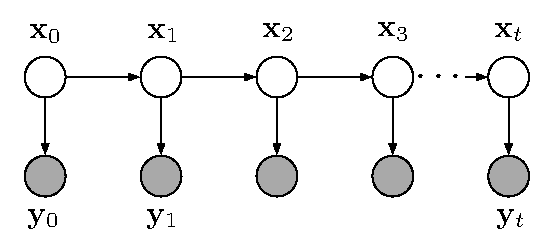
\includegraphics[scale=0.6]{HMM.pdf}
\end{tabular}
\end{figure}

\begin{itemize}
\item Time-Series (speech processing, tracking, ...)
\item In HMMs, the states $X_t$ are discrete.
\item In linear Gaussian SSMs, the states are real Gaussian vectors.
\item Both HMMs and SSMs can be represented as singly connected DAGs.
\item The forward–backward algorithm in hidden Markov models (HMMs), and the
Kalman smoothing algorithm in SSMs are both instances of belief propagation.
\end{itemize}

}


\section{Approximate Inference}

\begin{frame}{Approximate Inference}
\begin{itemize}
\item Few representative cases where exact inference is possible. Yet it can be very slow. 
\begin{itemize}
\item Discrete inference is always possible (just performing sums), but the Junction Tree Algorithm can be cumbersome.
\end{itemize}
\item In many other scenarios, exact inference is not even possible. We must therefore resort to \noteG{approximation techniques}.
\begin{enumerate}
\item Variational methods \& Mean Field approximations.
\item Loopy Belief Propagation, Approximate Message Passing, Expectation Propagation.
\item Sampling (Monte Carlo) methods. Importance Sampling.
\item Monte Carlo Markov Chain (MCMC), and includes as special cases Gibbs sampling and the Metropolis-Hasting algorithm.
\end{enumerate}
\item Approximate Inference is  \noteR{a huge topic}: see the references for more details. 
\end{itemize}
\end{frame}

\section{References}
\frame{
\frametitle{References}
\noteB{Books}
\begin{itemize}
\item  Christopher M. Bishop, Pattern Recognition and Machine Learning, Ed. Springer. Chapters 8-11.
\item David Barber, Bayesian Reasoning and Machine Learning. Chapters 1-7.
\item Kevin P. Murphy, Machine Learning: A Probabilistic Perspective. Chapters 10, 11, 18-24.
\end{itemize}

\noteG{Articles}:
\begin{itemize}
\item  Kevin P. Murphy, A Brief Introduction to Graphical Models and Bayesian Networks, 1998 (online).
\item Sam Roweis \& Zoubin Ghahramani, 1999. A Unifying Review of Linear Gaussian Models, Neural Computation 11(2) (1999) pp.305-345 
\item C. Huang and A. Darwiche, 1996. "Inference in Belief Networks: A procedural guide", Intl. J. Approximate Reasoning, 15(3):225-263. 
\item M. I. Jordan, Z. Ghahramani, T. S. Jaakkola, and L. K. Saul, 1997. "An introduction to variational methods for graphical models."
\item D. Heckerman, 1996. "A tutorial on learning with Bayesian networks", Microsoft Research tech. report, MSR-TR-95-06. 
\end{itemize}
}

\section{Software}

\begin{frame}{Software for Graphical Models}
\begin{itemize}
\item BUGS and WinBUGS: inference via Gibbs sampling, not very scalable
\item HUGIN: widely used, commercial, focus on exact inference
\item \noteG{Kevin Murphy’s Bayes Net Toolbox}: Matlab, widely used
\item Microsoft’s Infer.NET: advanced scalable libraries implementing factor graph
propagation, EP, and variational message passing.
\item Jeff Bilmes’ GMTK: very good at HMMs and related time series models
\end{itemize}
\end{frame}

\frame{
\frametitle{A personal library}

\begin{itemize}
\item My personal website \url{https://github.com/olmosUC3M/Inference-and-Learning-in-discrete-Bayesian-Networks.git} 
\item Not really scalable. The focus is on teaching through practice over small example using Python's notebooks. 
\item Easy to interpret and extend.
\item Open Source.
\end{itemize}


}


\end{document}

%%% Local Variables:
%%% mode: latex
%%% TeX-master: t
%%% End:
